\documentclass[12pt]{article}
\usepackage[utf8]{inputenc}
\usepackage[T1]{fontenc}
\usepackage{ dsfont }
\usepackage{amsfonts}
\usepackage{amssymb}
\usepackage{amsmath}
\usepackage{amsthm}
\usepackage{fancyhdr}
\usepackage{appendix}
\usepackage{mathptmx}
\usepackage{anyfontsize}
\usepackage{t1enc}
\usepackage{graphicx}
\usepackage{fancyhdr}
\usepackage{setspace}
\usepackage{float}

\usepackage[export]{adjustbox}
\usepackage{multicol}
\usepackage{array}
\setlength{\columnsep}{1cm}
\usepackage[a4paper,left=2cm,right=2cm,top=2cm,bottom=2cm]{geometry}
\usepackage{xcolor}
\usepackage{caption}
\usepackage{subcaption}

\usepackage{listingsutf8}
\lstset{inputencoding=utf8/latin1}
\usepackage[french]{babel}


\pagestyle{fancy}
\renewcommand\headrulewidth{1pt}
\renewcommand\footrulewidth{1pt}
\fancyhead[L]{Algorithme Numérique}
\fancyhead[R]{Théo Cliquot \& Valérian Capon} 
\fancyfoot[C]{
\includegraphics[scale =.12]{./img/prepisima.png}}
\fancyfoot[R]{{\Large \thepage}}
\fancyhead[C]{\rightmark}

\definecolor{darkWhite}{rgb}{0.94,0.94,0.94} 
\lstset{
  literate=
  {á}{{\'a}}1 {é}{{\'e}}1 {í}{{\'i}}1 {ó}{{\'o}}1 {ú}{{\'u}}1
  {Á}{{\'A}}1 {É}{{\'E}}1 {Í}{{\'I}}1 {Ó}{{\'O}}1 {Ú}{{\'U}}1
  {à}{{\`a}}1 {è}{{\`e}}1 {ì}{{\`i}}1 {ò}{{\`o}}1 {ù}{{\`u}}1
  {À}{{\`A}}1 {È}{{\'E}}1 {Ì}{{\`I}}1 {Ò}{{\`O}}1 {Ù}{{\`U}}1
  {ä}{{\"a}}1 {ë}{{\"e}}1 {ï}{{\"i}}1 {ö}{{\"o}}1 {ü}{{\"u}}1
  {Ä}{{\"A}}1 {Ë}{{\"E}}1 {Ï}{{\"I}}1 {Ö}{{\"O}}1 {Ü}{{\"U}}1
  {â}{{\^a}}1 {ê}{{\^e}}1 {î}{{\^i}}1 {ô}{{\^o}}1 {û}{{\^u}}1
  {Â}{{\^A}}1 {Ê}{{\^E}}1 {Î}{{\^I}}1 {Ô}{{\^O}}1 {Û}{{\^U}}1
  {œ}{{\oe}}1 {Œ}{{\OE}}1 {æ}{{\ae}}1 {Æ}{{\AE}}1 {ß}{{\ss}}1
  {ű}{{\H{u}}}1 {Ű}{{\H{U}}}1 {ő}{{\H{o}}}1 {Ő}{{\H{O}}}1
  {ç}{{\c c}}1 {Ç}{{\c C}}1 {ø}{{\o}}1 {å}{{\r a}}1 {Å}{{\r A}}1
  {€}{{\EUR}}1 {£}{{\pounds}}1, 
  backgroundcolor=\color{darkWhite},
  breakatwhitespace=true,
  breaklines=true,
  captionpos=b,
  commentstyle=\color{red},
  deletekeywords={...},
  escapeinside={\%*}{*)},
  extendedchars=true,
  keepspaces=true,
  keywordstyle=\color{blue},
  language=C,
  morekeywords={*,...},
  showspaces=false,
  showstringspaces=false,
  showtabs=false,
  stepnumber=1,
  stringstyle=\color{gray},
  tabsize=4,
  title=\lstname,
}

\lstdefinestyle{frameStyle}{
  basicstyle=\footnotesize,
  numbers=left,
  numbersep=20pt,
  numberstyle=\tiny\color{black}
}


\begin{document}


\begin{figure}[!htb]
  \begin{minipage}{0.5\textwidth}
    \centering
    
\includegraphics[width=.7\linewidth]{./img/prepisima.png}
    \caption{ ISIMA }\label{fig-ISIMA}
  \end{minipage}\hfill
  \begin{minipage}{0.5\textwidth}
    \centering
    
\includegraphics[width=.7\linewidth]{img/UCA.jpeg}
    \caption{Université de Clermont-Ferrand}\label{fig-UCA}
  \end{minipage}
\end{figure}



\vspace{5cm}
\begin{center}


  \color{red} {\fontsize{50}{60}\selectfont  Compte Rendu Algorithme Numérique}

  \vspace{0.5cm}
  \color{gray}
  \rule{0.6\linewidth}{1mm}

  \vspace{0.5cm}
  
  \color{red} {\huge Gauss, Choleski, Jacobi et Gauss-Seidel}

  \color{gray}
  \rule{0.6\linewidth}{1mm}
  
  \vspace{0.5cm}

  \color{black}
  Réalisé par : Théo Cliquot et Valérian Capon
  
  \vspace{0.5cm}
  
  En : Prep'ISIMA 1 (voir la figure ~\ref{fig-ISIMA} et et la figure ~\ref{fig-UCA})

  \vspace{0.5cm}
  
  Travail à rendre pour le: 24/10/2020
  
  \newpage

  \doublespacing
  \color{blue}
  \tableofcontents
  \listoffigures
  \color{black}
  \doublespacing
  \vspace{2.5cm}

\end{center}

\newpage


\section{Choleski}

J'ai seulement mit 2 chiffre après la virgule pour avoir une meilleur lisibilité dans le compte rendu et tester plus facilement les résultats ce qui peut des fois arrondir une erreur dans le calcul. Cependant cela n'empêche pas de voir quelques erreurs (comme dans Gauss Seidel)

\subsection{Rappel rapide de la méthode}



\begin{multicols}{2}

  La méthode de choleski permet de résoudre le système $A*x = B$ ( A étant une matrice carrée de taille n , x une matrice colonne inconnue que l’on essaie de trouver et B une autre matrice colonne.


  Pour ce faire on simplifie la matrice A sous la forme $R^{-1}*R$ (R étant une matrice triangulaire supérieure de taille n). Ce qui permet de transformer le système en $R^{-1}*R*x = B$ ou encore $R^{-1}*y = B$ avec $R*x = y$, C’est 2 équations deviennent beaucoup plus faciles à résoudre du faites que R et $R^{-1}$ sont triangulaires.


  Cependant la méthode de Choleski n’est possible que pour les matrices défini strictement positives et symétrique, en effet si ce n’est pas le cas pour la dernière on aura une racine carrée avec une valeur négatif ( ce qui est impossible sur $\mathds(R)$).

\end {multicols}

\subsubsection{Exemple}

Prenons la matrice A:$
  \begin{pmatrix}
 
    1 & 1 & 1 \\

    1 & 2 & 2 \\

    1 & 2 & 3 \\

  \end{pmatrix}
  $

  \vspace{0.3cm}
  
  R est la matrice A après Choleski. On définit i la ligne qu'on regarde actuellement et j la colonne. Dans un premier temps avec la formule \ref{Eq_Choleski1}

  \begin{equation}
    \label{Eq_Choleski1}
    r_{i i} = a_{i,i} - \sum_{j = 1}^{i-1} r_{j i}^2 
  \end{equation}
  
 Soit = $r_{1 1} = \sqrt{1} = 1 $ seulement si $a_{1,1} - \sum_{j = 1}^{i-1} r_{j i}^2 > 0 $ (sinon la méthode de choleski est impossible). On a donc R =
$
\begin{pmatrix}
 
    1 & x & x \\

    0 & x & x \\

    0 & 0 & x \\

  \end{pmatrix}
  $

   \vspace{0.2cm}
  
  Pour tout les autres elements sur la même ligne qui suivent on applique la formule \ref{Eq_Choleski2}:

  \begin{equation}
    \label{Eq_Choleski2}
    r_{i,j} = (a_{i j} - \sum_{k = 1}^{i-1} r_{k i} * r_{k j}) / r_{i i}
  \end{equation}


 Ainsi : $ r_{1 2} = 1$ et $ r_{1 3} = 1$ Ce qui nous donne pour R : $
\begin{pmatrix}
 
    1 & 1 & 1 \\

    0 & x & x \\

    0 & 0 & x \\

  \end{pmatrix}
  $

  Si on continue à appliquer c'est 2 méthodes ligne par ligne on obtindra à la fin R = $
 \begin{pmatrix}
 
    1 & 1 & 1 \\

    0 & 1 & 1 \\

    0 & 0 & 1 \\

  \end{pmatrix}
  $

\vspace{1cm}

\subsection{Présentation du programme (fonction dans \ref{Func_choleski})}

\begin{multicols}{2}

  La fonction \texttt{Choleski()} va suivre le même principe que vu au dessus. Pour cela elle va prendre en argument une tableau 2D de float \textit{matA} de taille \textit{taille} (taille étant aussi un argument) (dans notre exemple la matrice A) et une autre matrice 2D carrée  \textit{C1} de taille  \textit{taille} (notre matrice R dans l'exemple).
  cette fonction va renvoyer un entier : soit 0 ou 1. 0 représentant une erreur durant l'exécution de la méthode et 1 un bon fonctionnement du programme.

  Cette fonction va dans un premier temps parcourir chaque ligne. Dans chacune de ces lignes il va appliquer les 2 formules vu juste avant. La première formule ()\ref{Eq_Choleski1}) va être appliquer pour les éléments de la diagonale et à chaque fois on va vérifier si $a_{1,1} - \sum_{j = 1}^{i-1} r_{j i}^2 > 0$. Dans le cas contraire on arrête l'algorithme en renvoyant 0.Si ce n'est pas le cas on continue en appliquant cette fois ci la seconde formule (\ref{Eq_Choleski2}) et ceux pour tout les éléments dans les colonnes suivantes ( et en restant toujours dans la même ligne), c'est ce que fait la seconde boucle \texttt{for}. Ensuite il nous suffit d'appliquer la formule tout en faisant attention qu'on ne divise pas par 0 (dans ce cas on arrête le programme et on renvoie 0).
  
  Pour tout ce qui concerne les fonctions autour de choleski, la plupart servent à allouer dynamiquement des matrices 2D (avec malloc) ou à les libérer, à afficher des matrices 2D ou colonnes, à remplir les matrices soit aléatoirement (en respectant 70\% de 0 pour la matrice creuse) soit définies (comme Hilbert,Lehmer ...).
  
  La seule fonction un peu plus complexe permet de résoudre Ax = b que l'on appelle 2 fois : une fois pour résoudre $R^{-1}*y=matB$ et la seconde $R*x = y$. Pour cela la fonction va résoudre la première ou dernière ligne du système (en fonction de si on à rentré  $R^{-1}$ ou $R$). Puis elle va descendre (ou remonter) en utilisant les résultats précédents.
  

\end{multicols}

\subsection{Présentations de jeux d'essais pertinents}



On observe dans les matrices test que seuls 4 d’entre elles peuvent être transformer via l’algo de choleski (les 2 Hilbert, Lehmer et Moler), 

La matrice de Franc est assez intéressantes car elle pourrait être résolu par choleski si il n’existait pas la règle $ a_ij = 0 si i \geq j+2 $  et elle donnerait une matrice triangulaire uniquement 
composé de 1 (comme la matrice de l'exemple).

Moler donne aussi une matrice après Choleski assez particulière puisque qu’elle est à ça diagonale formée de 1 et le reste de -1. De plus comme elle est bien symétrique elle résout l’équation sans aucun problème (exemple avec une matrice de taille 3 (image \ref{Img_choleskiPreuveAlea})). Dans le cas des matrices creuses l'algorithme de Choleski ne marche que dans de rare cas en effet entre le fait que la matrice généré aléatoirement n'est pas forcément symétrique, définie strictement positive ou le faite qu'on peut rencontrer pendant l'exécution de choleski une division par 0 rends l'obtention d'une matrice faisable assez rare.

\newpage
\begin{figure}[H]
  \centering
    \begin{minipage}{0.6\textwidth}
      \centering
      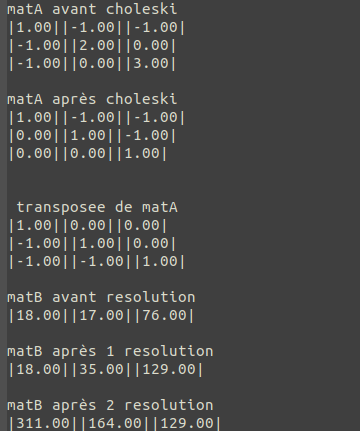
\includegraphics[width=1\linewidth]{img/choleskiPreuveAlea}
      \caption{Un exemple en utilisant la matrice de Moler}\label{Img_choleskiPreuveAlea}
    \end{minipage}\hfill
    \begin{minipage}{0.3\textwidth}
      311*1 - 164 – 129 = 18;
      
      -311 + 2*164 = 17;
      
      -311+129*3 = 76
      \end{minipage}
\end{figure}

Une erreur d'arrondie peut apparaître, en effet pour une meilleure lisibilité les variables dans les matrices ont était limitait à 2 chiffres après la virgule, ainsi si le résultat s'étend sur 3 chiffre après la virgule des erreurs vont apparaître. 

\subsection{Commentaires des jeux d'essais}

Il est assez facile de remarquer avec le temps d'exécution de choleski qu'elle n'est pas de complexité linéaire (en fonction de la taille du tableau) . Cependant on a un temps d'éxécution correctes (un peu plus d'une demi seconde pour un tableau de taille 1000 comme le montre la Figure~\ref{Img_choleskiTemps1000}).Il a était dit dans le cours que l'algorithme de Choleski est de complexité $n^3/3$. Pour le vérifier on calcule le nombre d'opérations effectué par l'algorithme avec un tableau de taille 5 et de taille 100. On obtient pour le premier 55 opérations 338350 pour le second. ce qui est plus que attendu (41 et 333334). Cependant on reste dans une complexité temporelle avec un ordre de grandeur de $n^3$ (si on essaie de trouver avec $n^4$ on à $5^4/11.5 \simeq 55$ mais $100^4/11.5 \simeq 8695652 \neq 333334$)

\begin{figure}[H]
  \centering
  \begin{subfigure}{1\textwidth}
    \centering
    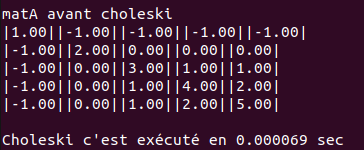
\includegraphics[width=0.5\linewidth]{img/choleskiTemps5}
    \caption{taille 5}\label{Img_choleskiTemps5}
  \end{subfigure}
  \begin{subfigure}{.8\textwidth}
    \centering
    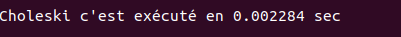
\includegraphics[width=0.75\linewidth]{img/choleskiTemps100}
    \caption{taille 100}\label{Img_choleskiTemps100}
  \end{subfigure}
  \begin{subfigure}{.8\textwidth}
    \centering
    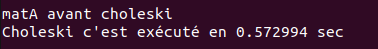
\includegraphics[width=0.75\linewidth]{img/choleskiTemps1000}
    \caption{taille 1000}\label{Img_choleskiTemps1000}
  \end{subfigure}
  \caption{Temps d'exécution avec des matrices de Moler de différentes tailles}
  \label{Fig_choleskiTemps}
\end{figure}




On peut aussi facilement observer que la méthode de Choleski est stable nottament avec un écart de 10\% (Image~\ref{Img_choleskiEcart1} et ~\ref{Img_choleskiEcart2} )

\begin{figure}[H]
  
  \begin{subfigure}{.5\textwidth}
    \center
    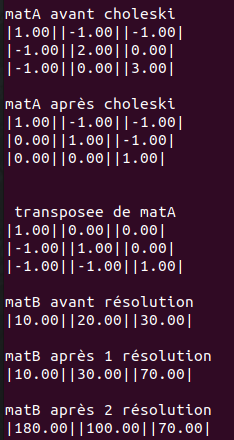
\includegraphics[width=0.8\linewidth]{img/choleskiEcart2}
    \caption{matB = \{10 20 30\}}\label{Img_choleskiEcart1}
  \end{subfigure}%
  \begin{subfigure}{.5\textwidth}
    \center
    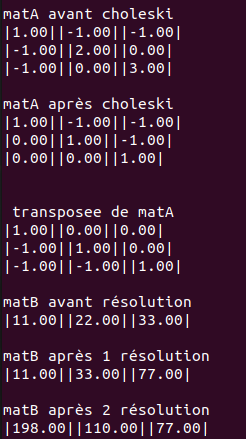
\includegraphics[width=0.8\linewidth]{img/choleskiEcart1}
    \caption{matB = \{11 22 33\}}\label{Img_choleskiEcart2}
  \end{subfigure}
\caption{Preuve de la stabilité pour Choleski}
\label{Fig_choleskiTemps}
\end{figure}

On a bien : $ 198 = 180*1.1 ; 110 = 100*1.1 ; 77 = 70*1.1$

\subsection{Conclusion Algorithme}
\begin{multicols}{2}


Choleski permet de trouver la bonne réponse comme gauss (par rapport au méthode indirectes comme Jacobi et Gauss Seidel) Cependant elle possède trois différences majeures avec Gauss. De 1 elle à une complexité moins élevé que Gauss : $n^3/3 \leq 2n^3/3$. Cependant et c’est la seconde et troisième différence elle a besoin de règles très précise pour fonctionner, en effet la matrice \textit{matA} doit être symétrique et définie positive, Ce qui limite beaucoup les matrices possibles. De plus on est obliger de créer un autre tableau 2D pour sauvegarder R, ce qui peut être négligeable si A est de petite taille mais peut se réveler bien plus problématique si à l'inverse A est de grande taille. Il est donc assez intéressant d’utiliser choleski lorsque c’est possible et si une matrice supplémentaire de même taille que A ne va pas surcharger la mémoire. 

\end{multicols}

\section{Gauss-Seidel}


\subsection{Rappel rapide de la méthode}



\begin{multicols}{2}

  Gauss Seidel comme Jacobi est une méthode itérative,c’est à dire qu’elle va s’approcher de la bonne solution mais pas forcément trouver la réponse exacte du système $Ax=B$. Cependant pour cela il faut que Gauss Seidel converge, c'est à dire soit A est diagonale dominante soit a est définis strictement positive. La méthode de Gauss Seidel consiste a appliquer Jacobi mais dans chaque itérations on utilise les résultats précédent.
  
  \subsubsection{Exemple}

  

\end {multicols}

Prenons la matrice A:$
  \begin{pmatrix}
 
    5 & 2 & -1 \\

    1 & 6 & -3 \\

    2 & 1 & 4 \\

  \end{pmatrix}
  $ La matrice B:$
  \begin{pmatrix}
 
    6 \\

    4 \\

    7 \\

  \end{pmatrix}
  $ Prenons ensuite comme point de départ P =$
  \begin{pmatrix}
 
    0 \\

    0 \\

    0 \\

  \end{pmatrix}
  $ et une marge d'erreur de 0.15 (ce qui est une grosse marge surtout pour un ordinateur mais elle permet de ne pas trop faire d'itérations.)


  Comme dit précédemment la méthode de Gauss Siedel suit la même logique que Jacobi. Le seul point qu'il n'ont pas en commun et le faite que Gauss Seidel va utiliser directement les nouvelles solutions trouvés dans l'itération.
  Ainsi prenons un systéme avec 3 inconnu $x_1 ; x_2 $ et $ x_3 $. Pour une certaine itération k, la première formule de Jacobi et de Gauss Seidel pour calculer $x_1^{k}$ vont être la même, ils vont tous les deux utiliser $x_2^{k-1}$ et $x_3^{k-1}$. Cependant à partir de la seconde formule Gauss Seidel ne va non pas utiliser $x_1^{k-1}$ comme Jacobi mais il va plutôt utiliser $x_1^k$, et ainsi de suite.
  
  On peut retrouver cette différence dans l'équation de Gauss Siedel (Formule (\ref{Eq_GS})) :

  \begin{equation}
    \label{Eq_GS} 
    x_i^k = \frac{1}{a_{i i}} * (b_i - \sum_{j<i} a_{i j} * x_j^k - \sum_{j > i} a_{i,j} * x_j^{k-1}).  
  \end{equation}

  Lorsqu'on regarde la deuxième $\sum$ dans cette formule on se rends compte que c'est exactement pareil que Jacobi, la seule différence vient donc des inconnus avant i (la première $\sum$) correspondant aux variables calculé avant dans l'itération.

  Ainsi si on reprends notre exemple. On obtient lors de la première itérations $P_1$ =$
  \begin{pmatrix}
 
    1.200 \\

    0.467 \\

    1.033 \\

  \end{pmatrix}$

  Seconde itérations $P_2$ =$
  \begin{pmatrix}
 
    1.220 \\

    0.980 \\

    0.895 \\

  \end{pmatrix}$

  
   Troisième itérations $P_3$ =$
  \begin{pmatrix}
 
    0.987 \\

    0.950 \\

    1.019 \\

  \end{pmatrix}$

  
  Quatrième itérations $P_4$ = $
  \begin{pmatrix}
 
    1.024 \\

    1.006 \\

    0.9866 \\

  \end{pmatrix}
  $
\vspace{0.2cm}

On va regarder si notre résultats pour l'itération 4 est bien compris dans la marge d'erreur, pour ça on va regarder si $A*p_4 - B \simeq 0$

\vspace{0.1cm}

On trouve : $\begin{pmatrix}
 
    0.145 \\

    0.100 \\

    0.000 \\

  \end{pmatrix}
  $

  \vspace{0.1cm}
  Toutes les valeurs de cette matrice sont $\leq$ à 0.15 donc notre résultats est compris de la marge d'erreur. 

\subsection{Présentation du programme (fonction dans \ref{Func_GS})}

\begin{multicols}{2}
Comme pour Choleski, Bon nombre de fonctions sont réutilisés (allocation d'une matrice 2D, affichaged'une matrice2D ...) La seule qui est rajouté est une fonction permettant de calculer rapidement le produit matriciel entre une matrice 2D et une matrice colonne (pour calculer la marge d'erreur).


La fonction Gauss Seidel va prendre plusieurs arguments en entrés. nottament 3 matrices : une matrice carrée 2D \texttt{matA}, une matrice colonne \texttt{matB}, une autre matrice colonne \texttt{valeurActuelle} toute de taille \texttt{taille} (qui est aussi un argument). Et enfin un float \texttt{erreurAccepté} qui correspond à la marge d'erreur.
Comme pour la fonction \texttt{Choleski}, Gauss Seidel retourne 1 si tout c'est bien passée et qu'il à trouver une solution respectant la marge d'erreur. Sinon il retourne 0 (nottament si il a fait trop d'itérations pour éviter une boucle infini ou qu'il y a une division par 0 à un moment).
La fonction de Gauss Seidel se compose d'une boucle while qui va continuer tant que l’une de ces deux conditions n’est pas vérifié :
\end{multicols}

\begin{itemize}
\item La fonction à dépassé un nombre de boucle autorisé (pour éviter la boucle infinie).
\item Le résultat obtenu est assez proche de la solution (dépend de la marge d'erreur).
\end{itemize}

\begin{multicols}{2}
A l'intérieur de cette boucle (qui correspond a une itération) On va appliquer la formule au dessus en écrasant à chaque fois \texttt{valeurActuelle}. Une fois qu'on à parcourue et modifié entièrement \texttt{valeurActuelle}. On réalise le même test vu dans l'exemple pour vérifier si notre résultat et compris dans la marge d'erreur et ceux en calculant $A*x$ grâce à une fonction extérieur qu'on stock dans matA\_X, une matrice colonne alloué. Si oui on arrête la boucle là ( 2eme condition vérifié), sinon on continue.
A la sortie de la boucle, un \texttt{if} sépare les 2 cas possibles pour la sortie de la boucle. Si la sortie de la boucle est dû à la première condition on arrête la function qui renvoie 1, sinon la fonction renvoie 0 car elle à finit sans problème. Dans les 2 cas on libère matA\_X pour éviter de gaspiller de la mémoire.
\end{multicols}

\subsection{Présentations de jeux d'essais pertinents}

Il y a 3 matrices test dans les 9 présentes qui respectent les conditions de Gauss Seidel (Moler, Lehmer et Franc). 
Exemple avec la matrice de Lehmer de taille 3:

\newpage

\begin{figure}[H]
  \begin{minipage}{0.4\textwidth}
    \centering
    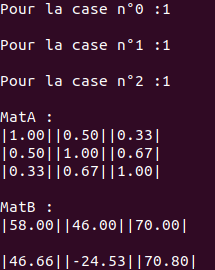
\includegraphics[width=1\linewidth]{./img/GSPreuveAlea}
    \caption{Un exemple en utilisant la matrice de Lehmer}\label{Img_GSPreuveAlea}
  \end{minipage}\hfill
  \begin{minipage}{0.5\textwidth}
    
    46,66 - 24,53*1/2 + 0,33*70,80 = 57.759
    
    46,66*0,5 – 24,53 + 0,67*70,80 = 46,236
    
    46,66*0,33 – 24,53*0,67 + 70,80 = 69,7627
 
  \end{minipage}
\end{figure}

 On observe que les résultats obtenu sont assez proches mais pas forcément égales. Ce qui est logiques puisque on accepte une marge d'erreur. Si on veut avoir des calculs plus précis il faudrait encore baisser notre marge d'erreur (et aussi afficher plus de chiffres après la virgule), ce qui implique plus d'itérations et donc un temps d'exécution plus long.
        
\subsection{Commentaires des jeux d'essais}

On remarque assez vite que le temps d' exécution n'est pas influencé par la taille des tableaux seulement, mais plus par le nombre d'itérations. En effet une matrice de taille 100 peut très bien prendre 1 itération (si notre point de départ est la solution) alors qu'une matrice de taille 5 va en prendre 250. Cependant la taille joue comme même un rôle car plus la matrice est grande, plus les itérations vont prendre de temps. Ainsi la complexité ne peut pas être calculé avec la taille de la matrice seulement, et de même avec seulement l'itération. (voir image (\ref{Img_GSTemps1}) et (\ref{Img_GSTemps2}))

\begin{figure}[H]
  
  \begin{subfigure}{.5\textwidth}
    \center
    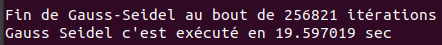
\includegraphics[width=1\linewidth]{img/GSIt1}
    \caption{taille de 125}\label{Img_GSTemps1}
  \end{subfigure}%
  \begin{subfigure}{.5\textwidth}
    \center
    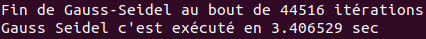
\includegraphics[width=1\linewidth]{img/GSIt2}
    \caption{même taille ... et pourtant un écart important}\label{Img_GSTemps2}
  \end{subfigure}
\caption{Temps exécution ainsi que le nombre d'itérations selon la taille}
\label{Fig_GSTemps}
\end{figure}

Si la matrice que l'on passe à l'entrée n'est pas diagonales dominantes où défini strictement positive, la méthode de Gauss Seidel ne va jamais converger ce qui va entraîner dans notre algorithme une fin de boucle non pas car on à trouver une solution mais pour éviter une boucle infini. On va aussi arrêter notre fonction si on divise par 0. Ces 2 critères rendent beaucoup de matrices creuses invalides. 

En ce qui concerne la stabilité on remarque aussi assez rapidement que Gauss Siedel est stable (voir image (\ref{Img_GSEcart1}) et (\ref{Img_GSEcart2}))


\begin{figure}[H]
  
  \begin{subfigure}{.5\textwidth}
    \center
    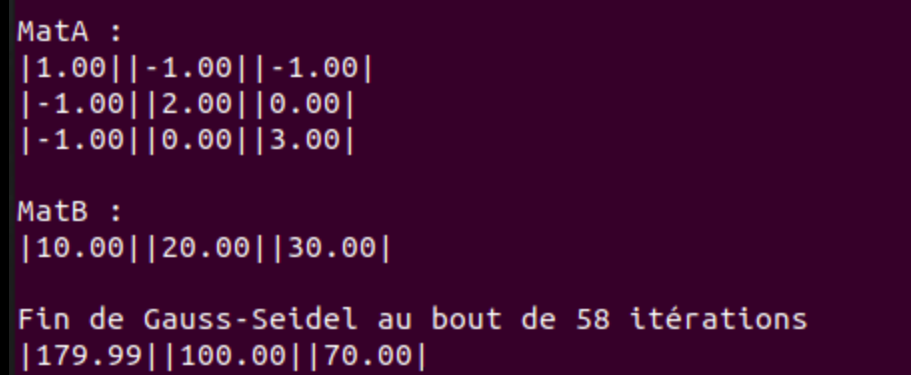
\includegraphics[width=1\linewidth]{./img/GSEcart1}
    \caption{matB = \{10 20 30\}}\label{Img_GSEcart1}
  \end{subfigure}%
  \begin{subfigure}{.5\textwidth}
    \center
    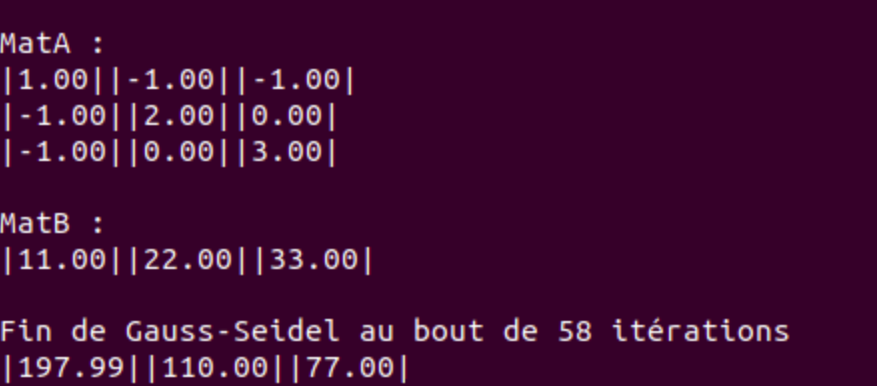
\includegraphics[width=1\linewidth]{img/GSEcart2}
    \caption{matB = \{11 22 33\}}\label{Img_GSEcart2}
  \end{subfigure}
\caption{Preuve de la stabilité pour Gauss Siedel}
\label{Fig_GSEcart}
\end{figure}

Si on ne prends pas en compte l'erreur au centième pour la première case de matB (179.99 $\simeq$ 180.00 et 197.99 $\simeq$ 198.00) on remarque tout de suite que c'est le même résultat que choleski. Donc Gauss Seidel est très très proche d'être stable (pour ne pas dire totalement).

\subsection{Conclusion Algorithme}

Gauss Seidel converge plus rapidement que Jacobi et il est plus large dans ses possibilités que Jacobi. Cependant on n’est pas sûr de trouver la réponse exacte (elle peut être très proche mais à 0,0.....01 près) ce qui est un désavantage par rapport au méthode non itérative tel Gauss ou Choleski. Cependant en ce qui concerne qui est le plus rapide entre les méthodes itératives et les directes est assez flou et on ne peut pas être sûr à 100\%.

En ce qui concerne les matrices creuses. La plupart ne sont pas valides car la fonction Gauss Seidel va diviser par 0 au bout d'un moment, si jamais il n'y a aucune division il faut encore que la matrice \texttt{matA} soit à diagonale dominante ou défini strictement positive, ce qui limite encore plus les choix.



\newpage
\appendix
\section{Fonction Choleski}
\label{Func_choleski}

\begin{lstlisting}

  // Cette fonction applique la méthode de choleski sur la marice matA en enregistre le réultat dans la matrice C1
  // Renvoie 1 (true) si l'algorithme c'est passé sans aucun problème, 0 (false) sinon.
  int Choleski(float ** matA,float ** C1, int taille)
  {
    
    /* matA correspond à notre matrice A dans le système Ax = B
    C1 est la matrice obtenue après que Choleski est travaillé avec matA
    taille représente la longueur de la matrice carrée A et C1 */
    
    for (int i = 0; i < taille; i++) //On parcours chaque ligne de la matrice matA
    {
      float t = matA[i][i];
      for(int l = 0; l<i ; l++)
      {
        t -= pow(C1[l][i],2);
      }
      // Si t inférieure à 0, alors on renvoie 0 (erreur);
      if(t <= 0)
      {
        printf("Algorithme de Choleski impossible\n");
        return 0;
      }
      // Sinon on peut continuer d'appliquer Choleski sans problème
      else
      {
        C1[i][i] = sqrtf(t);
        for(int j = i+1;j < taille;j++)
        {
          float s=0;
          for (int l = 0; l < i; l++)
          {
            s += C1[l][i] * C1[l][j] ;     
          }
          // De même si on divise par 0 Choleski renvoie une erreur
          if(C1[i][i] == 0)
          {
            printf("Division par 0\n");
            return 0;
          }
          else
          {
            C1[i][j] = (matA[i][j] - s)/C1[i][i];
          }
        }
      }
    }
    return 1;
  }

\end{lstlisting}

\vspace{0.5cm}

\section{Fonction Gauss-Siedel}
\label{Func_GS}

\begin{lstlisting}

// Cette fonction calcul la solution de matA*X = matB en fontion d'une erreurAccepté et d'un tableau contenant les valeurs de recherches, puis stock le résultat dans ce dernier tableau.
// Renvoie 1 (true) si la fonction n'a rencontré aucun problème 0 (false) sinon avec un message d'erreur 
int Gauss_Seidel(float  ** matA, float* matB, int taille, float erreurAccepte, float* valeurActuelle)
{

  /* matA et matB sont les matrices qui écrivent l'équation Ax = B (matA = A, matB = B) matA étant une matrice Carrée et matB une matrice colonne de longueur taille.
     erreurAccepté est la valeur influant sur la marge d'erreur
     valeuActuelle et le point de départ, à chaque itérations valeurActuelle se rapprochera de x (la solution) */

  
  // matA-X et le produit entre matA et notre résultat actuelle, cette matrice va permettre de confronter les résultats obtenu avec les vrais résultats
  float * matA_X = malloc(sizeof(float)*taille);

  // les 2 int qui suivent servent comme test d'arrêt, stop permet d'arrêter la boucle au bout de 100 itérations et valeurProche test si nos résultats sont cohérents (avec une marge d'erreur défini par erreurAccepte)
  int stop = 0;
  int valeurProche = 0;
  
  // Tant que l'un de nos test d'arrêt n'est pas vérifié.
  while (stop < 1000000000 && valeurProche == 0 )
    {
      
      valeurProche = 1;
      //Pour chaque ligne du système
      for(int i = 0; i < taille;i++)
	{
	  
	  // Permet d'éviter les divisions par 0.
	  if(matA[i][i] == 0)
	    {
	      printf("Division par 0\n");
	      // On libère matA_X puisque on en a plus besoin
	      free(matA_X);
	      return 0;
	    }
	  
	  float s = 0;

	  for (int j = 0; j < taille;j++)
	    {
	      if( i != j)
		{
		  s -= matA[i][j] * valeurActuelle[j];
		}
	    }
	  valeurActuelle[i] = (matB[i] + s)/matA[i][i] ;
	}
      
      produitDeAParX(matA_X,matA,valeurActuelle,taille);

      // Cette boucle vérifie si notre résultat et proche de celui attendu (1 si oui 0 sinon)
      for(int i = 0; i < taille;i++)
	{
	  if (fabs(matA_X[i] - matB[i]) > erreurAccepte)
	    {
	      valeurProche = 0;
	    }
	}
      stop++;
    }

  // On libère matA_X puisque on en a plus besoin
  free(matA_X);

  // On retourne faux si on arrête la boucle non pas car le résultat est proche mais à cause du nombre d'itérations important
  if(stop == 1000000000)
    {
      printf("Arrêt de la boucle par sécurité\n");
      return 0;
    }
  printf("Fin de Gauss-Seidel au bout de %d itérations\n",stop);
  return 1;
}

\end{lstlisting}



\begin{lstlisting}
  void sauvegarde(taquin t)
  {
    int num = 0;
    char nomSauvegarde[12];
    FILE * f;
    printf("Sauvegarde en cours \n");
    sprintf(nomSauvegarde,"sauv_%d.txt",num);
    while((f = fopen(nomSauvegarde, "r")))
    {
      fclose(f);
      num++;
      sprintf(nomSauvegarde,"sauv_%d.txt",num);
    }
    fclose(f);
    f = fopen(nomSauvegarde,"w+");
    if(f == NULL)
    {
      perror("ERREUR CREATION FICHIER");
    }
    printf("Sauvegarde du taquin dans le fichier : %s\n",nomSauvegarde);
    for (int i = 0;i<t.taille*t.taille;i++)
    {
      
      fprintf(f,"%d",t.tab[i/t.taille][i%t.taille]);
      if(i%t.taille != t.taille-1)
      {
        fputc(' ',f);
      }
      else
      {
        fputc('\n',f);
      }
    }
    fclose(f);
  }
\end{lstlisting}




\end{document}